\begin{figure}
  \centering
  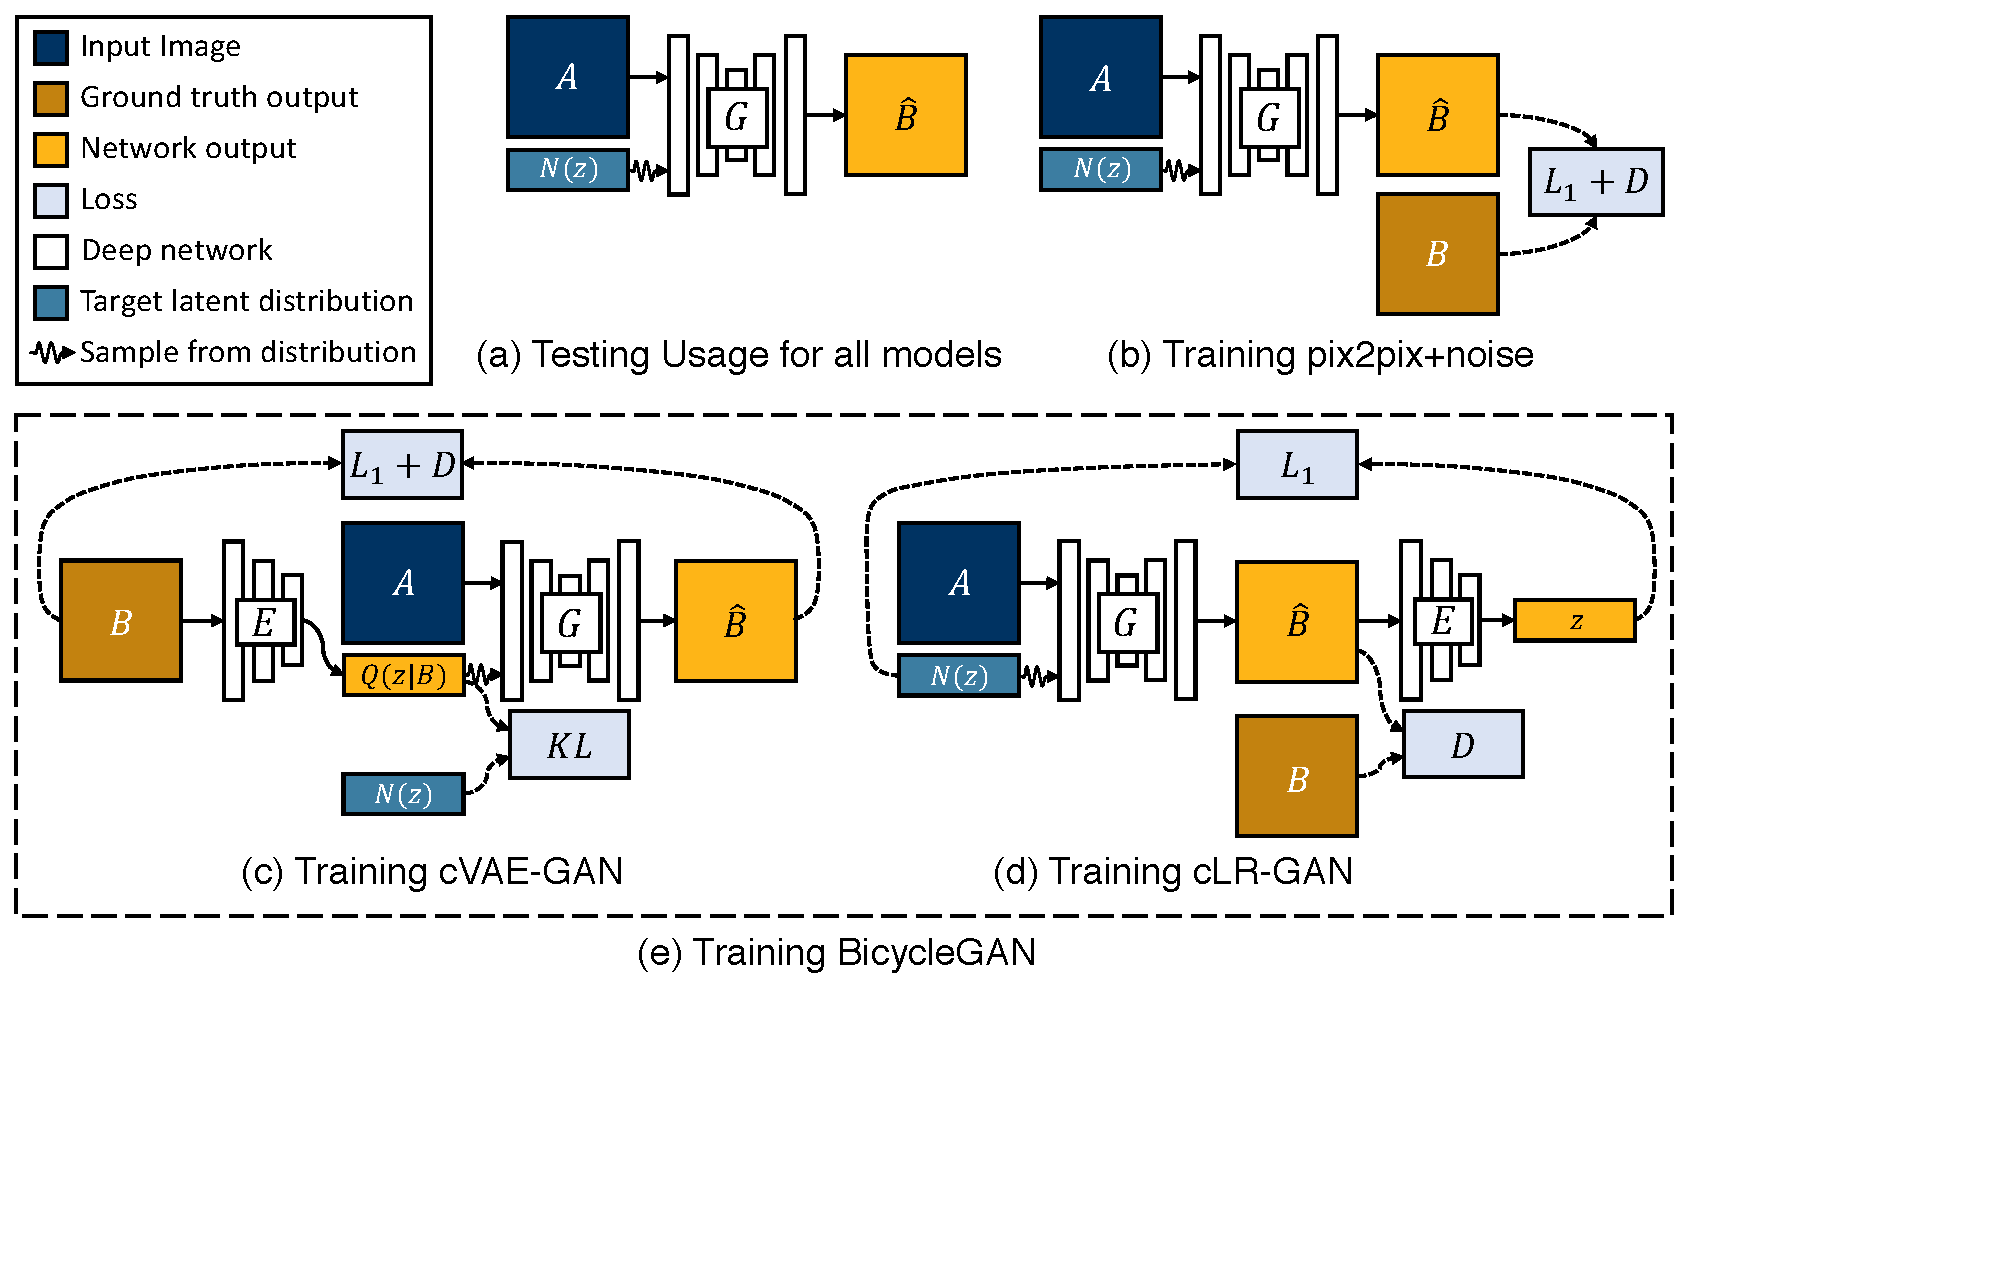
\includegraphics[width=1.\linewidth]{imgs/fig2.pdf}
\caption{\small \textbf{Overview}: (a) Test time usage of all the methods. To produce a sample output, a latent code $\mathbf{z}$ is first randomly sampled from a known distribution (e.g., a standard normal distribution). A generator $\G$ maps an input image $\mathbf{A}$ (blue) and the latent sample $\mathbf{z}$ to produce a output sample $\mathbf{\hat{B}}$ (yellow). (b) \ppn~\citep{isola2016image} baseline, with an additional ground truth image $\mathbf{B}$ (brown) that corresponds to $\mathbf{A}$. (c)  \cvaegan (and \cae) starts from a ground truth target image $\mathbf{B}$ and encode it into the latent space. The generator then attempts to map the input image $\mathbf{A}$ along with a sampled $\mathbf{z}$ back into the original image $\mathbf{B}$. (d) \cinfogan randomly samples a latent code from a known distribution, uses it to map $\mathbf{A}$ into the output $\mathbf{\hat{B}}$, and then tries to reconstruct the latent code from the output. (e) Our hybrid \bicycle method combines constraints in both directions.
}
\vspace{-5mm}
\label{fig:fig2}
\end{figure}

\section{Related Work}

\paragraph{Generative modeling}
Parametric modeling of the natural image distribution is a challenging problem. Classically, this problem has been tackled using restricted Boltzmann machines~\citep{smolensky1986information} and autoencoders~\citep{hinton2006reducing,vincent2008extracting}. 
% Variational autoencoders~\citep{kingma2013auto} enable test-time sampling by 
Variational autoencoders~\citep{kingma2013auto} provide an effective approach for modeling stochasticity within the network by reparametrization of a latent distribution at training time.
A different approach is autoregressive models~\citep{efros1999texture,van2016pixel,oord2016conditional}, which are effective at modeling natural image statistics but are slow at inference time due to their sequential predictive nature.
Generative adversarial networks~\citep{goodfellow2014generative} overcome this issue by mapping random values from an easy-to-sample distribution (e.g., a low-dimensional Gaussian) to output images in a single feedforward pass of a network. During training, the samples are judged using a discriminator network, which distinguishes between samples from the target distribution and the generator network.
GANs have recently been very successful~\citep{denton2015deep,radford2015unsupervised,donahue2016adversarial,dumoulin2016adversarially,reed2016generative,zhao2016energy,zhu2016generative,arjovsky2017wgan,zhang2016stackgan,xi2016infogan}. Our method builds on the conditional version of VAE~\citep{kingma2013auto} and InfoGAN~\citep{xi2016infogan} or latent regressor~\citep{donahue2016adversarial,dumoulin2016adversarially} models by jointly optimizing their objectives. We revisit this connection in Section~\ref{sec:finalMethod}.

\paragraph{Conditional image generation} All of the methods defined above can be easily conditioned. While conditional VAEs~\citep{sohn2015cvae} and
%PixelCNN~\cite{van2016conditional},
autoregressive models~\citep{oord2016conditional,van2016pixel} have shown promise~\citep{walker2016uncertain,xue2016visual,guadarrama2017pixcolor}, image-to-image conditional GANs have lead to a substantial boost in the quality of the results. However, the quality has been attained at the expense of multimodality, as the generator learns to largely ignore the random noise vector when conditioned on a relevant context~\citep{pathakCVPR16context,sangkloy2017scribbler,xian2017texturegan,yang2016high,isola2016image,zhu2017unpaired}. 
In fact, it has even been shown that ignoring the noise leads to more stable training~\citep{mathieu2015deep,pathakCVPR16context,isola2016image}.

\paragraph{Explicitly-encoded multimodality}
One way to express multiple modes is to explicitly encode them, and provide them as an additional input in addition to the input image.
For example, color and shape scribbles and other interfaces were used as conditioning in iGAN~\citep{zhu2016generative}, pix2pix~\citep{isola2016image}, Scribbler~\citep{sangkloy2017scribbler} and interactive colorization~\citep{zhang2017real}. An effective option explored by concurrent work~\citep{ghosh2017multi, chen2017photographic,bansal2017pixelnn} is to use a mixture of models. Though able to produce multiple discrete answers, these methods are unable to produce continuous changes.
While there has been some degree of success for generating multimodal outputs in unconditional and text-conditional setups~\citep{goodfellow2014generative,nguyen2016plug,reed2016generative,dinh2016density,larsen2016vaegan}, conditional image-to-image generation is still far from achieving the same results, unless explicitly encoded as discussed above. 
In this work, we learn conditional image generation models for modeling multiple modes of output by enforcing tight connections between the latent and image spaces.
